\section{Μοντέλο Οντοτήτων/Συσχετίσεων}

\subsection{Γενική Περιγραφή}

Οι οντότητες είναι : οι Εκδήλωση, η Τοποθεσία, το Εισιτήριο, ο Καλλιτέχνης-Ομάδα ,ο
Διοργανωτής,τα Φυσικά σημεία προπώλησης , ο Διοργανωτής, η Κάρτα και ο
Χρήστης. Για κάθε εκδήλωση θα πρέεπι να καταγράφεται το όνομά της, το
είδος της, η ημερομηνία που διεξάγεται, η ώρα και το όνομα του
καλλιτέχνη-ομάδας.

\underline{Υποθέσεις:}
\begin{itemize}[noitemsep]
\item Ο κωδικός εκδήλωσης είναι μοναδικός για κάθε εκδήλωση. Καμιά άλλη εκδήλωση
οποιαδήποτε μέρα δεν μπορεί να πάρει τον ίδιο κωδικό.
\item Οι αριθμοί κάρτας για κάθε χρήστη είναι μοναδικοί. Δεν μπορεί
  ένας χρήστης να έχει 2 κάρτες με τον ίδιο αριθμο.
\item Κάθε εκδήλωση πρέπει να έχει ακριβώς έναν καλλιτέχνη - ομάδα 
  \end{itemize}

\subsection{Καθορισμός Οντοτήτων}

Παρακάτω φαίνονται οι οντότητες της \titlos, η περιγραφή τους καθώς
και κάποια γνωρίσματά τους.

\begin{center}
\begin{tabular}[]{|p{4cm}|p{10cm}|}
\hline
\textbf{Όνομα Οντότητας}   &  Εκδήλωση  \\ \hline 
\textbf{Περιγραφή}         &  Οντότητα που αποθηκεύονται οι εκδηλώσεις \\ \hline 
\textbf{Ιδιότητες}         &  Ισχυρή οντότητα \\  \hline               
\textbf{Γνωρίσματα}        &  \underline{Κωδικός εκδήλωσης} \\
                           &  Όνομα \\
            ~              &  Ύπαρξη Εισιτηρίου \\
             ~             &  Κοινό που απευθύνεται \\
              ~            &  Περιγραφή \\
                           &  Ημερομηνία \\
                           &  Ώρα έναρξης\\
 \hline
\end{tabular}
\vspace{0.3 cm}


\begin{tabular}[]{|p{4cm}|p{10cm}|}
 \hline
\textbf{Όνομα Οντότητας}   &  Μουσική εκδήλωση  \\ \hline 
\textbf{Περιγραφή}         &  Οντότητα που αποθηκεύονται οι μουσικές εκδηλώσεις \\ \hline 
\textbf{Ιδιότητες}         &  Ασθενής οντότητα \\  \hline               
\textbf{Γνωρίσματα}        &  Ύπαρξη θέσεων καθήμενων \\
                           &  Είδος \\
                           &  Opening act \\
 \hline
\end{tabular}
\vspace{0.3 cm}

\begin{tabular}[]{|p{4cm}|p{10cm}|}
\hline
\textbf{Όνομα Οντότητας}   &  Θέατρο \\ \hline 
\textbf{Περιγραφή}         &  Οντότητα που αποθηκεύονται οι θεατρικές εκδηλώσεις \\ \hline 
\textbf{Ιδιότητες}         &  Ασθενής οντότητα \\  \hline               
\textbf{Γνωρίσματα}        &  Ύπαρξη θέσεων VIP \\
                           &  Διάρκεια \\
\hline
\end{tabular}
\vspace{0.3 cm}

\begin{tabular}[]{|p{4cm}|p{10cm}|}
\hline
\textbf{Όνομα Οντότητας}   &  Αθλητική εκδήλωση \\ \hline 
\textbf{Περιγραφή}         &  Οντότητα που αποθηκεύονται οι αθλητικές εκδηλώσεις \\ \hline 
\textbf{Ιδιότητες}         &  Ασθενής  οντότητα \\  \hline               
\textbf{Γνωρίσματα}        &  Άθλημα \\
                           &  Ύπαρξη θέσεων VIP \\
                           
\hline
\end{tabular}
\vspace{0.3 cm}

\begin{tabular}[]{|p{4cm}|p{10cm}|}
\hline
\textbf{Όνομα Οντότητας}   &  Τοποθεσία \\ \hline 
\textbf{Περιγραφή}         &  Οντότητα που αποθηκεύονται οι τοποθεσίες των εκδηλώσεων \\ \hline 
\textbf{Ιδιότητες}         &  Ισχυρή οντότητα \\ \hline 
\textbf{Γνωρίσματα}        &  \underline{Κωδικός τοποθεσίας} \\
                           &  Όνομα \\
                           &  Εσωτερικός χώρος \\
                           &  Τηλέφωνο \\
                           &  Δίεύθυνση \\ 
                           &  Ύπαρξη υποδομών ΑΜΕΑ \\ 
                           & { \begin{tabular}[]{c|c}
                           
                           Κατάλογος τιμών            & μπύρα \\
                                                      & κρασί \\
                                                      & ποτό \\  
                           \end{tabular} }  \\
\hline
\end{tabular}
\vspace{0.3 cm}


\begin{tabular}[]{|p{4cm}|p{10cm}|}
\hline
\textbf{Όνομα Οντότητας} & Εισιτήριο                            \\ \hline 
\textbf{Περιγραφή}       & Οντότητα που αποθηκεύονται οι τιμές των
                             διαφόρων εισιτηρίων μιας εκδήλωσης \\ \hline 
\textbf{Ιδιότητες}       & Ασθενής οντότητα                      \\ \hline               
\textbf{Γνωρίσματα}      & Τύπος εισιτηρίου                     \\ \cline{2-2}
                         & Τιμή                                 \\ \hline
\end{tabular}

\vspace{0.3 cm}

\begin{tabular}[]{|p{4cm}|p{10cm}|}
\hline
\textbf{Όνομα Οντότητας} & Καλλιτέχνης-Ομάδα                         \\ \hline 
\textbf{Περιγραφή}       & Οντότητα που αποθηκεύονται οι καλλιτέχνες ή οι ομάδες \\ \hline 
\textbf{Ιδιότητες}       & Ισχυρή οντότητα                           \\    \hline           
\textbf{Γνωρίσματα}      & \underline{Κωδικός ερμηνευτή}             \\
                         & Ονοματεπώνυμο                             \\
           ~             & Καταγωγή                                  \\
\hline
\end{tabular}
\vspace{0.3 cm}

\begin{tabular}[]{|p{4cm}|p{10cm}|} 
 \hline
\textbf{Όνομα Οντότητας} & Καλλιτέχνης                               \\ \hline 
\textbf{Περιγραφή}       & Οντότητα που αποθηκεύονται οι καλλιτέχνες \\ \hline 
\textbf{Ιδιότητες}       & Ασθενής  οντότητα
                                                                     \\ \hline          
\textbf{Γνωρίσματα}      & Είδος                                     \\
                         & Ημερομηνία γέννησης
                                                                     \\ \hline 
\end{tabular}
\vspace{0.3 cm}

\begin{tabular}[]{|p{4cm}|p{10cm}|}
\hline
\textbf{Όνομα Οντότητας} & Ομάδα                                \\ \hline 
\textbf{Περιγραφή}       & Οντότητα που αποθηκεύονται οι ομάδες \\ \hline 
\textbf{Ιδιότητες}       & Ασθενής  οντότητα                      \\ \hline
\textbf{Γνωρίσματα}      & Όνομα υπευθύνου                      \\ \hline 
\end{tabular}
\vspace{0.3 cm}

\begin{tabular}[]{|p{4cm}|p{10cm}|}
 \hline
\textbf{Όνομα Οντότητας}   &  Φυσικά σημεία προπώλησης \\ \hline 
\textbf{Περιγραφή}         &  Οντότητα που αποθηκεύονται οι τρόποι αγοράς εισιτηρίων \\\hline 
\textbf{Ιδιότητες}         &  Ισχυρή οντότητα \\       \hline           
\textbf{Γνωρίσματα}        &  \underline{Κωδικός σημείου} \\
                           &  Όνομα \\
                           &  Τηλέφωνο \\
                           &  Διεύθυνση \\ 
\hline 
\end{tabular}
\vspace{0.3 cm}

\begin{tabular}[]{|p{4cm}|p{10cm}|}
\hline
\textbf{Όνομα Οντότητας}   &  Διοργανωτής \\ \hline 
\textbf{Περιγραφή}         &  Οντότητα που αποθηκεύονται τα στοιχεία
                             των διαφόρων διοργανωτών \\ \hline 
\textbf{Ιδιότητες}         &  Ισχυρή οντότητα \\  \hline                 
\textbf{Γνωρίσματα}        &  \underline{Κωδικός Διοργανωτή} \\
            ~              &  Όνομα εταιρίας \\
             ~             &  email \\
                           &  Τηλέφωνο \\
                           &  password \\
\hline
\end{tabular}
\vspace{0.3 cm}

\begin{tabular}[]{|p{4cm}|p{10cm}|}
\hline
\textbf{Όνομα Οντότητας}   &  Κάρτα \\ \hline 
\textbf{Περιγραφή}         &  Οντότητα που αποθηκεύονται οι πιστωτικές/χρεωστικές κάρτες \\ \hline 
\textbf{Ιδιότητες}         &  Ασθενής οντότητα \\  \hline                 
\textbf{Γνωρίσματα}        &  \underline{Αριθμός Κάρτας} \\
            ~              &  Κωδικός ασφαλείας \\
             ~             &  Διεύθυνση \\
\hline
\end{tabular}
\begin{tabular}[]{|p{4cm}|p{10cm}|}\\ \hline
\textbf{Όνομα Οντότητας}   &  Χρήστης\\ \hline 
\textbf{Περιγραφή}         &  Οντότητα που αποθηκεύονται οι χρήστες\\ \hline 
\textbf{Ιδιότητες}         &  Ισχυρή οντότητα \\  \hline                 
\textbf{Γνωρίσματα}        &  \underline{Κωδικός Χρήστη} \\
            ~              &  Ονοματεπώνυμο \\
                           &  email \\
                           &  password \\
\hline
\end{tabular}
\vspace{0.3 cm}

\end{center}
\subsection{Καθορισμός Συσχετίσεων}

Παρακάτω αναφέρονται οι συσχετίσεις της βάσης δεδομένων \titlos
\begin{center}
\begin{tabular}[]{|p{4cm}|p{10cm}|}
  \hline
  \textbf{Όνομα Συσχέτισης} & Η Μουσική Εκδήλωση είναι Εκδήλωση\\ \hline
  \textbf{Περιγραφή} & Κάθε εκδήλωση μπορεί να είναι Μουσική Εκδήλωση\\ \hline
  \textbf{Ιδιότητες} & Is-A  \\ \hline
\end{tabular}
\vspace{0.3 cm}

\begin{tabular}[]{|p{4cm}|p{10cm}|}
  \hline
  \textbf{Όνομα Συσχέτισης} & Το Θέατρο είναι Εκδήλωση\\ \hline
  \textbf{Περιγραφή} & Κάθε εκδήλωση μπορεί να είναι θέατρο\\ \hline
  \textbf{Ιδιότητες} & Is-A  \\ \hline
\end{tabular}
\vspace{0.3 cm}

\begin{tabular}[]{|p{4cm}|p{10cm}|}
  \hline
  \textbf{Όνομα Συσχέτισης} & Η Αθλητική Εκδήλωση είναι Εκδήλωση\\ \hline
  \textbf{Περιγραφή} & Κάθε εκδήλωση μπορεί να είναι Αθλητική Εκδήλωση\\ \hline
  \textbf{Ιδιότητες} & Is-A  \\ \hline
\end{tabular}
\vspace{0.3 cm}


\begin{tabular}[]{|p{4cm}|p{10cm}|}
  \hline
  \textbf{Όνομα Συσχέτισης}   & Εισιτήρια εκδήλωσης            \\ \hline
  \textbf{Περιγραφή}          & Μια εκδήλωση μπορεί να έχει διάφορους τύπους
                             εισιτηρίων με διάφορες τιμές.     \\ \hline
  \textbf{Ιδιότητες}          & Has-A                          \\ \hline
  \textbf{Λόγος πληθικότητας} & 1:n                            \\ \hline
  \textbf{Συμμετοχή}          & Μερική Συμμετοχή του Εκδήλωση  \\ \cline{2-2}
                              & Ολική Συμμετοχή του Εισιτήρια \\ \hline
  \textbf{Γνωρίσματα}         & -                              \\ \hline
\end{tabular}
\vspace{0.3 cm}

\begin{tabular}[]{|p{4cm}|p{10cm}|}
  \hline
  \textbf{Όνομα Συσχέτισης} & Δίδεται \\ \hline
  \textbf{Περιγραφή} & Κάθε εκδήλωση πρέπει να έχει 1 καλλιτέχνη ή ομάδα\\ \hline
  \textbf{Ιδιότητες} & Has-A  \\ \hline
  \textbf{Λόγος πληθικότητας} & n:1 \\ \hline
  \textbf{Συμμετοχή} & Ολική Συμμετοχή του Ερμηνευτή\\ \cline{2-2}
                     & Ολική Συμμετοχή του Εκδήλωση \\ \hline
  \textbf{Γνωρίσματα} & - \\ \hline
\end{tabular}
\vspace{0.3 cm}


\begin{tabular}[]{|p{4cm}|p{10cm}|}
  \hline
  \textbf{Όνομα Συσχέτισης} &Ο ερμηνευτής είναι ομάδα\\ \hline
  \textbf{Περιγραφή} & Ο ερμηνευτής μπορεί να είναι ομάδα\\ \hline
  \textbf{Ιδιότητες} & Is-A  \\ \hline
\end{tabular}
\vspace{0.3 cm}
\begin{tabular}[]{|p{4cm}|p{10cm}|}
  \hline
  \textbf{Όνομα Συσχέτισης} &Ο ερμηνευτής είναι καλλιτέχνης\\ \hline
  \textbf{Περιγραφή} & Ο ερμηνευτής μπορεί να είναι καλλιτέχνης\\ \hline
  \textbf{Ιδιότητες} & Is-A  \\ \hline
\end{tabular}
\vspace{0.3 cm}


\begin{tabular}[]{|p{4cm}|p{10cm}|}
  \hline
  \textbf{Όνομα Συσχέτισης} & Διεξάγεται\\ \hline
  \textbf{Περιγραφή} & Κάθε εκδήλωση πρέπει να έχει 1 τοποθεσία\\ \hline
  \textbf{Ιδιότητες} & Has-A \\ \hline
  \textbf{Λόγος πληθικότητας} & n:1 \\ \hline
  \textbf{Συμμετοχή} & Ολική Συμμετοχή του Εκδήλωση\\ \cline{2-2}
                     & Μερική Συμμετοχή του Τοποθεσία \\ \hline
  \textbf{Γνωρίσματα} & - \\ \hline
\end{tabular}
\vspace{0.3 cm}


\begin{tabular}[]{|p{4cm}|p{10cm}|}
  \hline
  \textbf{Όνομα Συσχέτισης} & Προπώληση \\ \hline
  \textbf{Περιγραφή} & Κάθε εκδήλωση μπορεί να έχει φυσικά μέρη που προπωλούνται εισιτήρια\\ \hline
  \textbf{Ιδιότητες} & Has-A \\ \hline
  \textbf{Λόγος πληθικότητας} & n:m \\ \hline
  \textbf{Συμμετοχή} & Μερική Συμμετοχή του Εκδήλωση \\ \cline{2-2}
                     & Μερική Συμμετοχή του Σημεία προπώλησης\\ \hline
  \textbf{Γνωρίσματα} & - \\ \hline
\end{tabular}
\vspace{0.3 cm}


\begin{tabular}[]{|p{4cm}|p{10cm}|}
  \hline
  \textbf{Όνομα Συσχέτισης} & Διοργανώνεται\\  \hline
  \textbf{Περιγραφή} & Κάθε εκδήλωση πρέπει να έχει διοργανωτή\\ \hline
  \textbf{Ιδιότητες} & Has-A \\ \hline
  \textbf{Λόγος πληθικότητας} & n:m \\ \hline
  \textbf{Συμμετοχή} & Mερική Συμμετοχή του Διοργανωτής \\ \cline{2-2}
                     & Μερική Συμμετοχή του Εκδήλωση \\ \hline
  \textbf{Γνωρίσματα} & - \\ \hline
\end{tabular}
\vspace{0.3 cm}

\begin{tabular}[]{|p{4cm}|p{10cm}|}
  \hline
  \textbf{Όνομα Συσχέτισης} & Μέθοδος πληρωμής\\  \hline
  \textbf{Περιγραφή} & Κάθε χρήστης μπορεί να έχει κάρτα\\ \hline
  \textbf{Ιδιότητες} & Has-A \\ \hline
  \textbf{Λόγος πληθικότητας} & n:m \\ \hline
  \textbf{Συμμετοχή} & Mερική Συμμετοχή του Χρήστης \\ \cline{2-2}
                     & Ολική Συμμετοχή του Κάρτα \\ \hline
  \textbf{Γνωρίσματα} & - \\ \hline
\end{tabular}
\vspace{0.3 cm}


%αλλαγμενη σχεση
\begin{tabular}[]{|p{4cm}|p{10cm}|}
  \hline
  \textbf{Όνομα Συσχέτισης}   & Αγορά                                                                  \\  \hline
  \textbf{Περιγραφή}          & Κάθε χρήστης μπορεί να αγοράσει εισιτήρια ηλεκτρονικά από την εφαρμογή \\ \hline
  \textbf{Ιδιότητες}          & Has-A                                                                  \\ \hline
  \textbf{Λόγος πληθικότητας} & n:m                                                                    \\ \hline
  \textbf{Συμμετοχή}          & Mερική Συμμετοχή του Χρήστης                                           \\ \cline{2-2}
                              & Μερική Συμμετοχή του Εκδήλωση                                          \\ \hline
  \textbf{Γνωρίσματα}         & Τύπος εισιτηρίου                                                       \\ \hline
\end{tabular}
\vspace{0.3 cm}



%νεα σχεση  %ποιος ο λογος πληθικοτητας;
% \begin{tabular}[]{|p{4cm}|p{10cm}|}
%   \hline
%   \textbf{Όνομα Συσχέτισης} & Πουλάνε\\  \hline
%   \textbf{Περιγραφή} & Τα σημεία προπώλησης πουλάνε εισιτήρια για την εκδήλωση\\ \hline
%   \textbf{Ιδιότητες} & Has-A ( Τριαδική)\\ \hline
%   \textbf{Λόγος πληθικότητας} & n:m \\ \hline
%   \textbf{Συμμετοχή} & Mερική Συμμετοχή του Σημεία Προπώλησης, Εκδήλωση \\ \cline{2-2}
%                      & Ολική Συμμετοχή του Εισιτήρια \\ \hline
%   \textbf{Γνωρίσματα} &  - \\ \hline
% \end{tabular}
% \vspace{0.3 cm}



\begin{tabular}[]{|p{4cm}|p{10cm}|}
  \hline
  \textbf{Όνομα Συσχέτισης} & Ενδιαφέρον \\  \hline
  \textbf{Περιγραφή} & Κάθε χρήστης μπορεί να αποθηκέυσει τις εκδηλώσεις που τον ενδιαφέρουν \\ \hline
  \textbf{Ιδιότητες} & Has-A \\ \hline
  \textbf{Λόγος πληθικότητας} & n:m \\ \hline
  \textbf{Συμμετοχή} & Mερική Συμμετοχή του Χρήστης \\ \cline{2-2}
                     & Μερική Συμμετοχή του Εκδήλωση \\ \hline
  \textbf{Γνωρίσματα} & - \\ \hline
\end{tabular}
\vspace{0.3 cm}

\end{center}


\subsection{Διάγραμμα Οντοτήτων/Συσχετίσεων}

\begin{figure}[H]
  \centering
  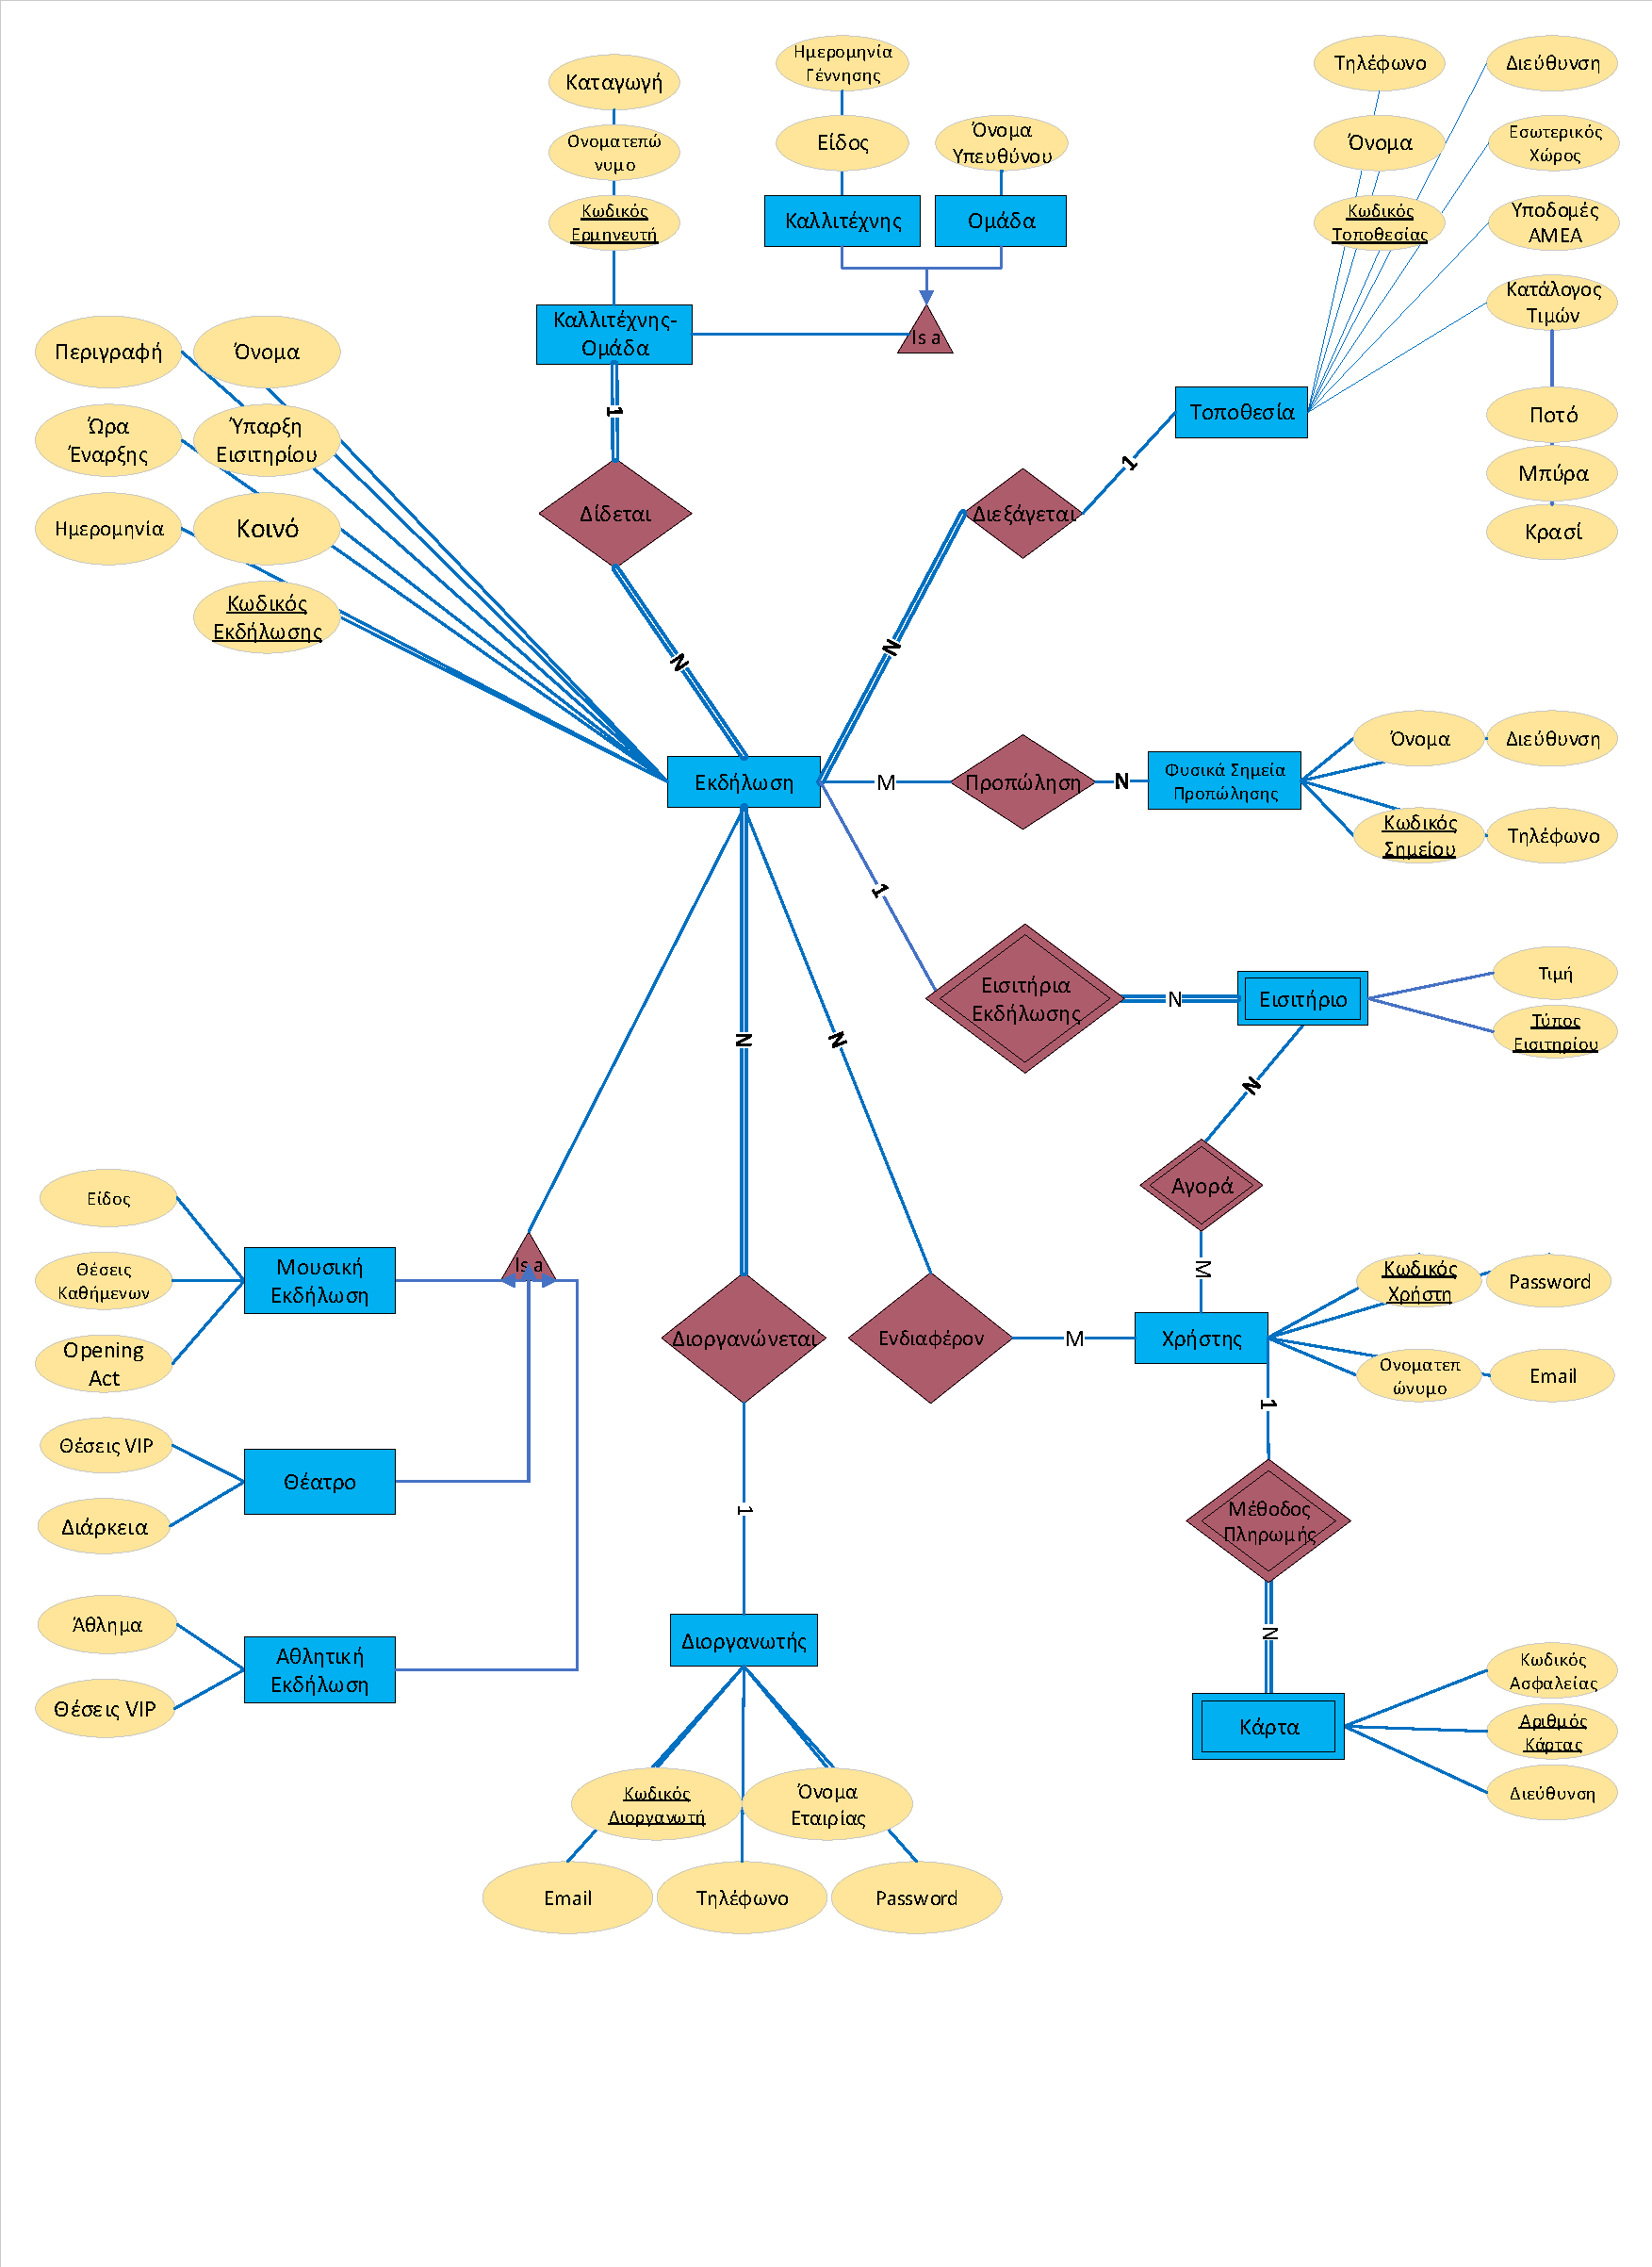
\includegraphics[width=.9\linewidth]{Entities.pdf}
  \caption{Διάγραμμα Οντοτήτων/Συσχετίσεων}
\end{figure}


%%% Local Variables:
%%% mode: latex
%%% TeX-master: "main"
%%% End:
